\documentclass[1p]{elsarticle}

\usepackage{lineno,hyperref}
\modulolinenumbers[5]
\usepackage[utf8]{inputenc}
\usepackage[spanish]{babel}
\usepackage{amsmath}
\usepackage{graphicx}
\usepackage{amsfonts}
\usepackage{amssymb}
\newtheorem{thm}{Teorema}
\newtheorem{lem}[thm]{Lema}
\newdefinition{rmk}{Definición}
\newproof{pf}{Demostración}
\newproof{pot}{Demostración del Teorema \ref{thm2}}
%%\bibliographystyle{IEEEannot}

%% `Elsevier LaTeX' style
\bibliographystyle{elsarticle-num}
%%%%%%%%%%%%%%%%%%%%%%%
\usepackage{setspace}  
\begin{document}

\begin{frontmatter}

\title{Mathematical model review of inmune competition in cancer dynamics}

%% Group authors per affiliation:
\author{Bartolomé Ortiz Viso}
\address{EDP de transporte\\Máster en Física y Matemáticas\\ Universidad de Granada\\17/01/2018}

\begin{abstract}
This work is a brief revision and study about the research article  \textbf{A mathematical model of inmune competition related to cancer dynamics}\cite{original} by \textit{Ilaria Brazzoli, Elena De Angelis and Pierre-Emmanuel Jabin}. My aim is to present its mains results, some technical highlights related to the mathematical proofs and comment about its implications and future research. Moreover I presents some basics concepts about kinetic theory for active particles in inmune competition situations that could be used in other topics if needed.
\end{abstract}

\begin{keyword}
 \texttt{kinetic theory for active particles} \sep \texttt{tumor-inmune competition}\sep \texttt{tumor dormancy} \sep \texttt{cell population}

\end{keyword}

\end{frontmatter}

\linenumbers

\section{Introducción}
\spacing{1.3}
 El desarrollo de la teoría cinética de partículas activas ha supuesto un gran avance para el descubrimiento de nuevos modelos matemáticos en el ámbito de la biología. Muchos de los ámbitos biológicos en los cuales el modelado matemático es una herramienta de reconocida necesidad, se han visto afectados por este desarrollo.


 Es necesario hacer hincapié en la diferencia elemental con teoría cinética clásica, que como vimos en nuestro curso es habitualmente aplicada en ámbitos físicos, donde se trabaja con partículas que interaccionan a niveles mecánicos y geométricos. En nuestro caso, sin embargo, estamos ante un contexto formado por un gran número de entidades interactivas llamadas partículas activas, en las que, a parte de influencia de variables geométricas o mecánicas es indispensable una variable de actividad, que caracteriza el sistema de vida específico que se modelará. Estas interacciones entre partículas no solo modifican el estado microscópico, si no que pueden generar comportamientos globales.

A menudo, nos encontramos en la literatura\cite{libro} que esta nueva teoría cinética puede incluir como casos especiales los modelos clásicos de la teoría cinética que también han formado parte de la asignatura de \textit{EDP de transporte y fluidos} a saber, las ecuaciones de Boltzmann y Vlasov.\\

Centrándonos en el tema central del trabajo, la teoría cinética de partículas supone un marco habitual en el desarrollo de modelos de competición inmune en los cuales no solo la proliferación de diferentes poblaciones de células son importantes si no también distintas cualidades o actividades que cada una de ellas presente.

Este es el caso del articulo que aquí se analiza: la dinámica tumoral, su interacción con el sistema inmune y otras poblaciones celulares. Esta competición supone una de las primeras barreras en las cuales se trata de reducir o suprimir comportamientos tumorales y, como se expone en \cite{bibid},juega un papel determinante en la supervivencia y metástasis de los tumores.

Debido a la multitud de factores biológicos implicados, es imprescindible un estudio multidisciplinar en el cual la creación de modelos matemáticos predictivos puede ayudarnos a comprender a que nos enfrentamos.



\section{Presentación del modelo}
El modelo a estudiar pretende describir una fase del desarrollo tumoral de la cual sabemos aun muy poco: la inmunovigilancia. Durante esta fase, el sistema inmune debe reconocer células tumorales durmientes, que pueden no presentar aun comportamiento tumoral y estar en un estado de alteración latente (dentro del cual habitualmente acumulan alteraciones y mutaciones). Estas células latentes, por este motivo, presentan una gran resistencia a ser eliminadas mediante tratamientos habituales, por lo que su comprensión puede ayudarnos a la hora de desarrollar nuevos tratamientos o comprender otras fases tumorales. 

Estudiamos un sistema formado por tres poblaciones de células que interactúan entre si en el marco de la teoría cinética de partículas: células endoteliales, células inmune y células tumorales, con indices $i=1,2,3$ y distribuidas de forma homogénea en el espacio. El modelo representará la forma de interactuar y auto-organizarse de estas tres poblaciones.

\paragraph{Principios del modelado}

Como comentábamos en la introducción, la teoría cinética de partículas activas nos permite enriquecer el modelo caracterizando de forma matemática actividad biológica celular. Esta caracterización se describe mediante una variable escalar $u\in I=[0,\infty]$, llamada \textit{variable de actividad}.

El significado de dicha variable debe especificarse para cada población en nuestro sistema:\begin{enumerate}
\item células endoteliales: capacidad de alimentación
\item células inmunitarias: activación 
\item células tumorales: progresión, cómo de lejos se encuentran las células de un estado sano.
\end{enumerate} 
La descripción del estado general del sistema en el tiempo $t\in[0,T]$ se define mediante la \textbf{función de distribución de una partícula generalizada} para cada población:
$$f_i=f_i(t,u)$$
para $i = 1,2,3$, generalmente dependiendo del tiempo $t$ y la actividad $u$.
Usando $f_i$ podemos pasar de un estudio microscópico a calcular cantidades microscópicas que caracterizan el comportamiento del sistema. Nos interesa los que se conocen como momentos de orden cero y uno:
$$
n_i(t)= n_i [f_i] (t) =\int_{0}^{+\infty} f_i (t, u) du,
$$
que se asocia a la densidad total o tamaño de población y,

$$A_i (t) = A_i [f_i] (t) =\int_{0}^{+\infty}uf_i(t,u),$$

que se asocia con la actividad de cada población.
En nuestro caso relacionaremos y analizaremos el comportamiento de $A_1, A_2 $ y $A_3$ éste último haciendo uso de su función de distribución $f_3$. Nuestro objetivo será buscar comportamientos en los que el sistema inmune llegue a un equilibrio de actividad, mientras que la actividad de las células tumorales vaya aumentando.

Como se describe en modelos similares de competicion inmunologica \cite{existencia}, $f_1$ y $f_2$ no son necesarias para analizar nuestro modelo, puesto que carecen de la información relevante al tener toda nuestra atencion centrada en el desarrollo de $f_3$   

\paragraph{Hipótesis del modelado}
\begin{enumerate}
	\item La proliferación de las células endoteliales ($A_1$) se ve afectada negativamente (destrucción celular) debido a la progresión de células tumorales. A su vez, se ve afectada positivamente por la propia reproducción celular. No se contemplan mas tipos de interacción.
	\item Las células inmunes tienden a relajar su actividad ($A_2$) hasta un \textit{estado centinela} asociado a una constante. Además la actividad tumoral provoca la actividad inmunológica.
	\item Las células tumorales proliferan según una función que depende de la progresión tumoral y las células inmunes provocan una destrucción de las células tumorales según su actividad.
\end{enumerate}
Recordamos que nuestra inquietud principal se corresponde con la evolución de la población de las células tumorales en cuestión de tiempo y actividad tumoral o progresión tumoral, con lo que serán esas las que describamos mediante una ecuación de transporte. Presentamos finalmente el modelo:
\begin{equation}
\frac{d}{dt}A_1=-A_1(t)A_3(t)+\alpha(A_1)A_1(t),
\label{a1}
\end{equation}
\begin{equation}
\frac{d}{dt}A_2=A_2^*-A_2(t)+A_3(t),
\label{a2}
\end{equation}
\begin{equation}
\partial_tf_3+\partial_uf_3=r(u)f_3(t,u)-A_2(t)f_3(t,u).
\label{a3}
\end{equation}
A esto debemos añadirle las condiciones iniciales:
\begin{equation}
A_1(0)=A_1^0,\textrm{ }A_2(0)=A_2^0,\textrm{ }f_3(t=0,u)=f_3^0(u).
\label{condiciones}
\end{equation}
y una condición de contorno para $f_3$, fundamentalmente representa que el origen de las células tumorales está en el propio tejido, así como que estas representan un aporte a  las células tumorales debido a la propia naturaleza de las células endoteliales.
 \begin{equation}
 f_3(t,0)=\beta A_1(t).
 \label{condicionesf}
 \end{equation}
\section{Resultados teóricos y descripciones técnicas}
En esta sección vamos a presentar los resultados puramente teóricos del articulo. No pretende ser un análisis exhaustivo de las pruebas contenidas en el mismo, si no un acercamiento a las demostraciones en el articulo expuestas así como a ciertas hipótesis o lemas que nacen necesariamente para el correcto tratamiento del modelo.

 Un análisis extenso de algunos modelos similares a este puede encontrarse en \cite{elvesier,existencia,libro,original,pdf,textolargo} de los cuales se pueden obtener algunas ideas relevantes a la hora de probar los resultados expuestos.

Las interpretaciones puramente biológicas de las hipótesis y los resultados pueden consultarse en la sección \ref*{inter}. Se decide así puesto que en gran parte de esta sección nos centraremos en resultados matemáticos técnicos.

El resultado principal y vertebral del artículo se centra en la existencia de un comportamiento asintótico de las soluciones bajo determinadas hipótesis.
Veamos primero cuáles son éstas:
\paragraph{Hipótesis}
\label{hipo}\begin{enumerate}[(i)]
	\item $\alpha \in L^\infty[0,+\infty)$, con $A_1^*>0$
	\item $r(u)\in L^\infty[0,+\infty)$ y $r(0)=0$
	\item $r(u)=R^*-(A/u)+O(1/u^2)$ cuando $u\rightarrow\infty$
\end{enumerate}
Presentamos los resultados:

 \begin{thm}
Suponiendo: \begin{equation}f_3^0(u)\geq0 \text{ y } \int_{0}^{+\infty}(1+u)f_0^3(u)du<\infty\label{cond}\end{equation}
Entonces existe al menos una solución $(A_1,A_2,A_3)$ para el problema de valores iniciales $(1)-(5)$ en el sentido de las distribuciones, tal que $(A_1,A_2)\in C([0,\infty))$ y $f_3\in L^1((1+u)du)$.
 \end{thm}
\paragraph{Comentarios}El teorema aparece sin demostrar en el artículo. Con los conocimientos adquiridos en el estudio de modelos de teoría cinética de partículas activas, planteo una posible vía de demostración basada en la información que tenemos. Es razonable que no sea la más sencilla o directa y aunque también se propone una alternativa no hay un consenso generalizado, en parte por las no linealidades que presenta el modelo.

En general las dos primeras ecuaciones del sistema no plantearían problema, la tercera pertence a una ecuación de evolución o transporte, de hecho podemos ver el \ref{a3} de la forma:
\begin{equation}
\partial_tf_3+\partial_uf_3-(r(u)-A_2(t))f_3(t,u))=0
\end{equation} 
Lo que equivale a una ecuación de transporte. Como queremos debilitar nuestras hipótesis iniciales (tengamos en cuenta que estamos trabajando con distribuciones) la prueba rigurosa podría pasar por debilitar el problema. Hemos dado varias estrategias a lo largo del curso para atacar este tipo de problemas. Podríamos tomar una solucion inicial de $A_2$ e insertarla dentro de \ref{a3} y actuar mediante un proceso iterativo. Leyendo gran parte de la bibliografía, presentamos un esquema de una posible demostración del resultado que he comprobado que se suele utilizar bastante:
\begin{itemize}
	\item Estimaciones a priori: Cualquier solución $f_3$ de la ecuación \ref{a3} en sentido débil debe satisfacer las estimaciones. En particular hablamos de que se debe satisfacer:
	$$ {\int_{0}^{+\infty}(1+u)f^3(u)du} <{\int_{0}^{+\infty}(1+u)f_0^3(u)du}<{\infty}$$
	Cota que se puede obtener de \ref{a3} si multiplicamos por una adecuada  función $\phi(u)$ e integramos por partes el término de transporte.
	\item Continuidad en tiempo: 
	Dadas $A_i \in L^\infty([0,T])$ demostrar que las soluciones débiles que satisfacen la cota pertenecen también a:
	$$C([0,T],L^1((1+u)du)), \forall T>0$$
	\item Estabilidad:
	Sea $f_3^n$ en el anterior espacio una secuencia de solución en el sentido de las distribuciones satisfaciendo la generalización de la estimación a priori uniformemente en n. Entonces cualquier limite débil de parciales convergentes pertenece a 
	$$C([0,\infty],L^1((1+u)du)), T>0$$
	y resuelve el sistema en el sentido de las distribuciones con las condiciones iniciales adecuadamente debilitadas.
	\item Existencia: Finalmente construimos una sucesión de soluciones aproximadas de nuestro sistema que satisface la estimaciones a priori. Tomamos límites débiles obtenemos soluciones para cualquier condición inicial que satisfaga nuestras hipótesis en $[0,T]$. Como las soluciones satisfacen las estimaciones uniformemente, podemos extender en tiempo la existencia.
\end{itemize}
 Este esquema en general es muy utilizado para probar resultados de existencia en el sentido de las distribuciones en casos de competición inmune \cite{pdf,existencia} aunque otros esquemas también son compatibles, como el de punto fijo \cite{textolargo} similar al que vimos en clase. Tanto el esquema como la cota de $f_3$ creo que parten de los anteriores artículos de los autores, pues suelen trabajar con ellas y probar similares resultados.
 
 

\begin{thm}
	Si $$sup_{\xi\in \mathbb{R}^+}\alpha(\xi)+A_2^*<R*$$
	donde $$R^*=sup_{u\in\mathbb{R}^+}r(u)$$
	entonces el unico equilibrio de nuestro sistema (1)-(5) es la solucion trivial:$A_1=0,\space A_2=A_2^*,\space f_3=0$. El equilibrio es inestable.
\end{thm}
\paragraph{Comentarios}La prueba de este teorema se lleva a cabo mediante reducción al absurdo. Supondremos por tanto la existencia de $A_1$,$A_2$, $f_3$ pertenecientes a una solución no trivial. La contradicción viene precisamente de las cotas. A partir de la solución que suponemos que existe, al ser de equilibrio:
\begin{equation}
0=-A_1(t)A_3(t)+\alpha(A_1)A_1(t),
\label{11}\end{equation}
\begin{equation}
0=A_2^*-A_2(t)+A_3(t),
\label{12}
\end{equation}
\begin{equation}
\partial_uf_3=r(u)f_3(t,u)-A_2(t)f_3(t,u).
\label{13}
\end{equation}
de \ref{11} obtenemos $A_3=\alpha(A_1)$ y de \ref{13} obtenemos resolviendo la ecuacion diferencial restante en u:
$$A_3=A_1\int_{0}^{\infty}ue^{R(u)-A_2u}du$$
con $R(u)=\int_{0}^{u}r(s)ds$
Si consideramos la integral como una función dependiente de $A_2$ podemos utilizar una herramienta que no hemos utilizado antes durante el curso: la transformada de Laplace.
La describimos brevemente:
\begin{rmk}[Transformada de Laplace]
	F se dice la \textbf{transformada de Laplace}  de una funcion f si:$$F(s) = \mathcal{L} \left\{f(t)\right\} =\int_{0}^\infty e^{-st} f(t)\,dt$$
	\end{rmk}
La transformada, gracias a sus propiedades, nos permite escribir $\frac{A_3}{A_1}=F(A_2)$ o, similarmente:
$A_2=F^{-1}(\frac{A_3}{A_2})$. Solo nos queda usar \ref{12}para hallar una ecuación para $A_1$. Usando las cotas de la hipótesis sobre los supremos, encontraremos que podemos escoger adecuadamente un número que no cumpla la ecuación. El resto de detalles técnicos están ampliamente explicados en \cite{original}, resaltamos aquí el uso de la resolución de ecuaciones más sencillas así como el conocimiento de la transformada de Laplace (que no hemos usado en la asignatura) para construir ecuaciones con buena regularidad e invertibles.

Finalmente vamos a comentar el último y más importante resultado:
\begin{thm}
	Suponiendo que la condición inicial cumple la condición \ref{cond}, entonces cuando $t\rightarrow\infty$ se tiene:
	\begin{enumerate}
		\item $A_1(t)\rightarrow0$;
		\item $n_3(t)\rightarrow0$;
		\item $A_2(t)\rightarrow R^*$ y $A_3(t)\rightarrow R^*-A_2^*$;
		\item $\exists L(u)\in L^1(du,\mathbb{R})$ y $\exists\phi(t)$de manera que $f_3$ con la adecuada normalización converge a $L(u)$
		$$\int_{\infty}^{\infty}f_3(t,u+t)\frac{e^{Alog(u+t)}}{\phi(t)}-L(u)du\leq\frac{c}{t}$$
		donde $c$ es constante y $A$ es la definida en la hipótesis \textit{(III)}
	\end{enumerate}\label{teorema3}
\end{thm}
La demostración del resultado se muestra integra en este trabajo, en este teorema se hace uso de dos lemas de acotación previos, en los cuales destacamos un paso que pudiera no quedar claro:
\begin{lem}
	Para la solución del problema planteado en (1)-(5) $A_2$ y $A_3$ están acotados.
\end{lem}
 \paragraph{Comentarios}La prueba de este teorema es bastante directa, en general basada en estimaciones realizadas sobre el sistema inicial. Destacamos la primera aseveración: \textit{Formalmente de \ref{a3} obtenemos:}
 $$\frac{d}{dt}A_3\leq R^*A_3+n_3-A_2A_3$$
Formalmente podemos comprobar la igualdad usando la multiplicación en \ref{a3} por u y la posterior integración del termino de transporte. La demostración rigurosa pasaría por tomar una sucesión de funciones $\psi_R(u)$ en $[0,R]$ y tomar límites. El procedimiento al completo está desarrollado en \cite{textolargo}.
\begin{lem}
	Para la solución del problema planteado en (1)-(5) tenemos:
	\begin{itemize}
		\item $\int_{0}^{t}A_2(s)ds\geq-k'+(R*-\epsilon)t; $
		\item $\int_{0}^{t}A_3(s)ds\geq-k''+(R*-\epsilon-A_2^*)t; $
	\end{itemize}
	donde $k' y k''>0$ y se verifica $max_{\xi\in\mathbb{R}^+}\alpha(\xi)+A_2^*-R^*<-2\epsilon$
\end{lem}
Basándonos en estos dos lemas, ya podemos proceder con la demostración en la que se basa el artículo:

\paragraph{Demostración Teorema 3}De la ecuación \ref{a1} obtenemos:
$$A_1(t)\leq A_1^0exp((max \alpha(\xi))t-\int_{0}^{t}A_3(s)ds)\leq A_1^0e^{-\xi t}e^{k''}$$
donde la última desigualdad la obtenemos gracias a el lema 5 y el Teorema 1 (en particular de la hipótesis de acotación). Gracias a esto podemos probar el primer apartado del teorema.
Para la segunda conclusion primero necesitamos una cota inferior para $A_3$.
Tomemos $\nu$ y $u_0$ tales que $\forall u>u_0$ , $r(u)\leq A_2^2 +2\nu$. Asumiendo que existe un intervalo temporal $[t_0 , t_1 ]$ dentro del cual $\nu / C<A_3 <\nu / 2, A_3 (t_0 ) = \nu / 2$ y $A_3 (t_1 ) = \nu / C$ con $C$ elegido mas adelante.

Notemos que en $[t_0 , t_1 ]$
$$\frac{d}{dt} A_2 \leq A_2^* +\nu / 2-A_2$$

aqui podemos utilizar la solución general para una ecuación diferencial :
$$A_2 (t)\leq A_2^* +\nu / 2+k e^{-(t-t_0 )}$$
Por otra parte como :
$$\frac{d}{dt}
A_3 \geq -kA_3
$$
tenemos de nuevo:
$$t_1 -t_0 \geq log C/k$$
Por tanto para $t>(t_0 +t_1 ) / 2$
\begin{equation}
A_2 (t)\leq A_2^* +\nu
\end{equation}
tomando un C lo suficientemente grande para que
$$e^{(log C)/(2k)} \geq 2k$$
Ahora, por la propia definición de $A_3$ si tomamos un $u_0>0$:
$$A_3 (t)\geq \widetilde{A_3} =\int_{u_0}^{\infty}uf_3 (t, u) du$$
Si integramos la ecuación \ref{a3} obtenemos:
$$\frac{d}{dt} \widetilde{A_3} \geq\int_{u_0}^{\infty}r(u)uf_3 -A_2 \widetilde{A_3} \geq(A_2^* +2\nu-A_2 ) \widetilde{A_3} \geq \nu \widetilde{A_3}$$
para  $t>(t 0 +t 1 ) / 2$. Esto significa que, resolviendo la ecuación diferencial:
$$A_3 (t_1 )\geq \widetilde{A_3} ((t_0 +t_1 ) / 2)e ^{\nu (t_1 -t_0 )/2}$$
Por \ref{a3}, tenemos para  $u\leq t$ 
$$f_3 (t, u)\leq A_1 (t -u)e^ku \leq ke^{ - \xi t} e^{ku}$$
gracias a la desigualdad del apartado (1). 
Por tanto, por contradicción si $(t_0 +t_1 ) / 2$ es lo suficientemente grande respecto a $u_0 , k, \nu$ y $\xi$:
$$A_3=A_3-\int_{0}^{u_0}uf_3du\geq A_3-\nu/2C\geq\nu/2C$$
Concluyendo tenemos:
$$A_3(t_1)\geq \frac{\nu}{2C}e^{(\nu logC)/(2C)}$$
y esto contradice $A_3 (t_1 ) =\nu / 2C $ si $C$ es elegido lo suficientemente grande como para tener
$$e ^{( \nu log C)/(2k)} >2$$
Esto supone que $ (t_0 +t_1 ) $no puede ser demasiado grande y por tanto$ A_3$ está acotado por abajo. 
Con esto demostrado vamos a por la parte (2) del teorema:
Definamos $l(t, u) = f 3 (t, t +u)$ de manera que por \ref{a3}, $l$ es la solución de la ecuación
$$\partial_t l = (r(t +u)-A 2 )l$$
y $l(t, -t) = \beta A_1 (t)$.
Consecuentemente:
$$l(t, u) = l(s, u) exp(\int_{s}^{t}(r(x+u)-A_2(x))dx).$$

Tomemos ahora  $u<t / 2$, entonces 
$$f_3(t,u)\leq f_3(t-u,0)exp(\int_{t-u}^{t}(r(u+s-t)-A_2(s))ds)$$
que lo volvemos a obtener de \ref{a3}.Usando de nuevo la primera acotación obtenemos:

$$f_3 (t -u, 0) = \beta A_1 (t -u)\leq ke^{ - \xi (t-u)} \leq ke^{ - \xi (t/2)}$$
Por tanto podemos resolver para obtener:
\begin{equation}f_3(t,u)\leq ke^{\xi t}exp(\int_{t-u}^{t}(r(s-t/2)-A_2(s))ds)
\label{24}
\end{equation}
Ahora si $t'<t$ y $v>t -t'$, tenemos
$$f_3 (t, v) = f_3 (t', v -t +t') exp(\int_{t'}^{t}(r(v+s-t)-A_2(s))ds)$$
de manera que si  $u<t / 2, t' = t -u$, y $v>u$, deducimos


\begin{equation}
\begin{split}
&f_3 (t, v) = f_3 (t-u,v-u) exp(\int_{t-u}^{t}(r(v+s-t)-A_2(s))ds)\\
&\geq f_3 (t-u,v-u) exp(\int_{t-u}^{t}(r(u+s-t)-A_2(s))ds)
\end{split} 
\end{equation}

Por la propia definición de $A_3$ , usando la desigualdad anterior  y \ref{24}, obtenemos las siguientes acotaciones:

\begin{equation}
\begin{split}
&A_3(t)\geq \int_{u}^{\infty}vf_3(t,u)dv\\
&\geq exp(\int_{t-u}^{t}(r(v+s-t)-A_2(s))ds)\int_{u}^{\infty}vf_3(t-u,v-u)dv\\
&\geq exp(\int_{t-u}^{t}(r(v+s-t)-A_2(s))ds)\int_{u}^{\infty}(v-u)f_3(t-u,v-u)dv\\
&\geq\frac{e^{\xi(t/2)}}{k}f_3(t,u)A_3(t-u)
\end{split} 
\end{equation}



y podemos deducir que:
\begin{equation}f_3 (t, u)\leq ke^{- \xi(t/2)}\frac{A_3 (t)}{A_3(t-u)}\leq k'e^{- \xi(t/2)}, \forall u\leq t/2
\label{25}
\end{equation}
por que hemos demostrado que $A_3$ estaba acotada inferiormente.
Retomando la definición de $n_3$ tenemos:

\begin{equation}
\begin{split}
&n_3=\int_{0}^{t/2}f_3du\int_{t/2}^{\infty}f_3du\leq\frac{t}{2}k'e^{-\xi(t/2)}+\frac{2}{t}\int_{0}^{\infty}uf_3du\\
&\leq k'e^{-\xi t}+(k'/t)A_3(t)
\end{split} 
\end{equation}

concluimos así el apartado 2 del teorema. Vamos con la penúltima parte:
De la ecuación \ref{a3}:
$$\frac{d}{dt}A_3 (t) =\int_{0}^{+\infty}
ur(u)f_3 (t, u) du-A_2 (t)A_3 (t)+n_3 (t) = R^* A_3 (t)-A_2 (t)A_3 (t)+\xi(t)$$
donde hemos definido $\xi(t)$ de la forma:
$$\xi(t) = n_3 (t)+\int_{0}^{+\infty}u(r(u)-R^* )f_3 (t, u) du$$
Ahora, de la 3º condición impuesta en Hipótesis, tenemos:
$$\xi(t)\leq n_3 +c\int_{0}^{\infty}f_3 (t, u) du\leq cn_3 (t)\leq c/t$$
donde para la ultima desigualdad hemos usado la cota (16).
Para el comportamiento asíntotico de $A_2$ y $A_3$ los autores utilizan un argumento de disipación. Para este fin deberemos comprobar como un funcional de Lyapunov tiende a cero. La forma en la que está definido en el artículo no deja pista sobre la forma en la cual lo han encontrado:
$$F(t) =(1/2)(R^* -A_ 2)^2 +\nu(A_2 -A_3 -A^*_2 )^2 +(R^* -A^*_ 2 ) log\frac{R^*-A^*_2}{A_3}+A_3-(R^*-A^*_2)$$

con $\nu$ pequeño. Por definición, si derivamos, obtenemos:

\begin{equation}
\begin{split}
&\frac{d}{dt}F(t)\leq  (R^*A_2 )^2 (1-\nu A_3 )^2 -\nu(A_2 -A_3 -A^*_ 2 )^2\\
&+\xi(t)((A_3 -A_2 -A^*_2 )+ (A_2 -R^* )+2\nu(A_3 -A_2 -A^*_2 ))\\
&\leq -(R^*A_2 )^2(1-1/(\nu A_3^2)-1/2)+\xi^2(t)(\frac{1}{2A_3^2}+\frac{3}{A_2^2}+12)\\
&-\nu(A_2-A_3-A_2^*)^2(1-\frac{\nu}{3}-\frac{\nu}{3})
\end{split} 
\end{equation}

En resumen hemos comprobado que:
$$\frac{d}{dt}F(t)\leq -cF+c'(\xi^2(t))$$
con c y c' constantes, por tanto$ F(t) \rightarrow 0$ as $t \rightarrow \infty$. Cerramos así la demostracion del apartado 3.
Antes de avanzar notemos la siguiente cualidad: si $|\xi(t)|\leq c/t$
entonces:
$$F(t)\leq\frac{c}{t^2}$$
Por último para terminar de probar el resultado completo, vamos con el apartado 4:
Definamos
$$
g(t, u) =f_3 (t, u+t)e^{A log(u+t)}, \forall u\geq-t$$
y cero en cualquier otro caso. De nuevo por la ecuacion \ref{a3}, tenemos:
\begin{equation}
\begin{split}
\partial_t g=(r(u+t)+A/(u+t)-A_2)g\\
=(r(u+t)+A/(u+t)-R^*)g+(R^*-A_2)g\\
=:a(u+t)g+b(t)g\\
=O(\frac{g}{(u+t)^2})+b(t)g
\end{split} 
\end{equation}





donde para la ultima estimación hemos usado fuertemente de nuevo el apartado 3 de las Hipótesis.
Sea $\phi(t)$ la solución del siguiente problema de Cauchy:
$$\left\{
\phi'(t)=b(t)\phi(t) \atop
\phi(0)=1
\right.$$
Por la anterior acotación que hicimos de $F(t)$  sabemos que si $|b(t)|\leq c / t$, por tanto:
$$\int_{0}^{t}|b(s)| ds\leq c log t$$
y
$$e^{-c log t} \leq\phi(t)\leq e^{c log t}$$
Ahora tomando $h(t, u) = (1 / \phi(t))g(t, u)$, de manera que $\partial_t h = a(u+t)h$, podemos usar:
\begin{lem}
	La función $h=h(.,u)$ pertenece a $L^1$ y verifica la condición de Cauchy, es decir, $t\geq s$:
	$$\int_{-\infty}^{+\infty}|h(t,u)-h(s,u)|du\rightarrow0$$ si $s,y\rightarrow +\infty$
\end{lem}
La demostración del lema no es trivial, aunque puede acometerse usando la propia definición de $h$, se puede consultar con tal fin \cite{original}.
Gracias a este lema, podemos decir que existe $L(u)\in L^1(du,\mathbb{R})$ tal que $h(t,u)\rightarrow L(u)$ en $L^1$ cuando $t\rightarrow\infty$ de hecho:
$$\int_{-\infty}^{+\infty}|h(t,u)-L(u)|du\leq\frac{c}{t}$$
Lo que concluye el resultado.

En general la demostración es puramente técnica, basada en el uso de las correctas acotaciones para cada término. 



\section{Interpretación biológica de hipótesis y resultados}\label{inter}
 En primer lugar,tratamos la adecuación de las hipótesis que imponemos en la sección de resultados teóricos. Estas hipótesis expresan la condición razonable de que hay un límite para la capacidad de reproducción tanto de las células endoteliales como de las células tumorales. 
 
 Particularmente, (I) expresa no sólo la acotación de en la reproducción, además ésta se puede entender como la tasa de reproducción de las células endotelilaes si no hay células tumorales. Esta tasa no puede crecer infinitamente y es razonable de que se aproximará a un equilibrio.
 
 Centrándonos en (II) es señalable también que el valor para $u=0$ sea $0$. Entendemos biológicamente esta hipótesis, a parte de como ya hemos apuntado, como que aquellas células recién mutadas a células cancerígenas aun no tenga capacidad multiplicativa como células propiamente tumorales. Esta delimitación es matemática y el modelo se desarrollaría de igual forma (incluido (\ref{condicionesf})) si el estado de célula tumoral reproductiva se alcanzase con otra cota.
 
 Finalmente sólo señalar que la elección de $(III)$ se hace acorde con la experiencia de los investigadores con el único requerimiento de la caída en las colas. Esta condición se hace necesaria en las pruebas pero carece a priori de significado biológico.
  
Llevando nuestra atención a la variable $f_3$, destacamos: la condición \ref{cond} impuesta en el resultado de existencia,  es consistente con los requisitos biológicos de las poblaciones celulares:
\begin{equation}
\begin{split}
&\int_{0}^{+\infty}(1+u)f_0^3(u)du<\infty\Rightarrow\\
&\Rightarrow\int_{0}^{+\infty}f_0^3(u)du<\infty \text{ y }\int_{0}^{+\infty}uf_0^3(u)du<\infty
\end{split} 
\end{equation}
Que nos viene a dar una acotación para la cantidad de células tumorales iniciales (segunda integral) y la capacidad de actividad de las mismas (tercera integral).

El resultado principal se establece en el Teorema \ref{teorema3} y se refiere al comportamiento asintótico del sistema. Comparando este modelo con otros modelos desarrollados en el mismo marco matemático de teoría cinética de partículas activas observamos cambios importantes. Por ejemplo, los analizados en \cite{textolargo,existencia} (que también han servido de base para realizar este trabajo) obtienen resultados de regresión de células tumorales debido a una acción efectiva del sistema inmune y el opuesto, con el estallido de las células con alta actividad tumoral y la inhibición progresiva del sistema inmune. 

Lo que tenemos ahora es un escenario diferente: observamos la evolución de la progresión de las células tumorales de tal manera que su número disminuye y su actividad puede mantenerse bajo control, aunque ésta no desaparece. Biológicamente entendemos que esta situación puede quedar caracterizada por un pequeño número de células tumorales con altos valores de actividad tumoral (medida por la variable $u$). Al mismo tiempo, el sistema inmune, después de  activarse, es capaz de volver a una situación muy cercana a la fisiológica, mientras que la actividad de las células endoteliales
disminuye a cero.

Este comportamiento es biológicamente relevante y puede asemejarse al que ocurre en la etapa de inmunovigilancia: el tumor proliferante se mantiene en números bajos y en una situación controlada en términos de población celular. El resultado analítico muestra una evolución
de la afectación de las células tumorales como una especie de "ondas viajeras" a través de la función $L(u)$. Esto resultados se verán más claros con las simulaciones numéricas de la siguiente sección.


\section{Simulaciones numéricas de casos concretos}
En esta parte voy a comentar brevemente algunos ejemplos de los analizados numéricamente en el artículo. 

Es de destacar que las simulaciones numéricas se hacen para arrojar algo más de información sobre $L(u)$ y sobre el comportamiento cualitativo en general. Se prueban también distintas condiciones iniciales y de contorno. 

Siguiendo las hipótesis se eligen una parábola como función de proliferación $\alpha(A_1)$ y una expresión de $r$:
$$r(u)=\frac{1}{a+\frac{1}{u}}$$
Así, tenemos $R^*=1$ y $A=1$. Además se supone que el valor centinela del sistema inmune corresponde a el valor inicial de $A_2=A_2^*$.
Usando un esquema de diferencias finitas resolvemos el problema $(1)-(5)$. Tras esto se calcula $\phi=\phi(t)$ como:
$$\int_{0}^{+\infty}f_3(t,u+t)e^{Alog(u+t)}du$$
Una vez obtenida esa cantidad computamos h(t,u) como sigue, que convergerá a $L(u)$ en $L^1(du,\mathbb{R})$ cuando $t\rightarrow\infty$:
$$h(t,u)=\frac{1}{\phi(t)}f_3(t,u+t)e^{Alog(u+t)}$$
Comentamos los dos casos tratados, correspondientes a a dos condiciones iniciales de $f_3$:
\begin{itemize}
	\item $f_3^0(u)=0$
	\item $f_3^0(u)=\text{Distribución de tipo Gaussiana}$
\end{itemize}
\begin{figure}
	\centering
	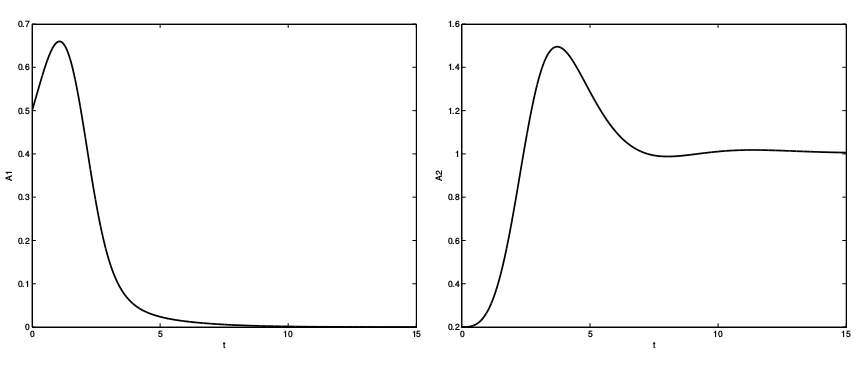
\includegraphics[width=1\textwidth]{test1A1A2.png}
	\caption{Representación de $A_1$ y $A_2$ en el primer caso}
	\label{fig:ejemplo2}
\end{figure}
\begin{figure}
	\centering
	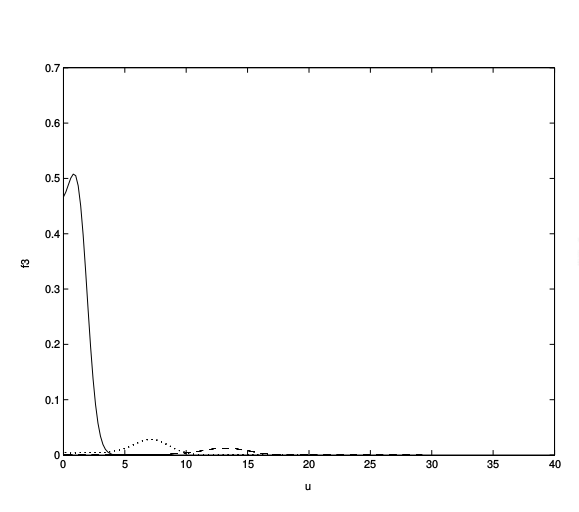
\includegraphics[width=1\textwidth]{test1F3.png}
	\caption{Comportamiento de $f_3$ en el caso 1 las lineas simbolizan la progresión temporal de $t=2$, $t=8$ y $t=14$ }
	\label{fig:ejemplo3}
\end{figure}
\begin{figure}
	\centering
	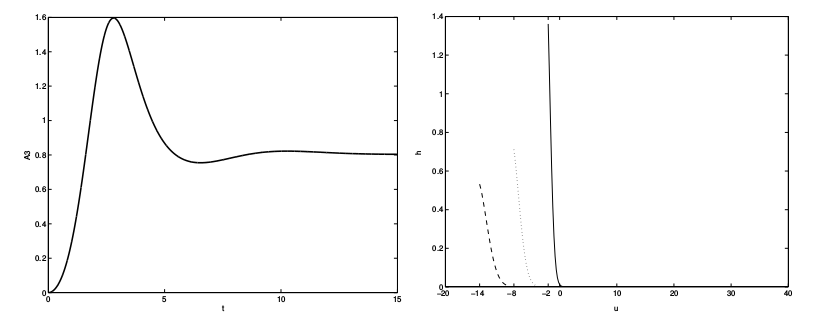
\includegraphics[width=1\textwidth]{test1A3H.png}
	\caption{Comportamiento de $A_3$ y $h$ en el caso 1}
	\label{fig:ejemplo4}
\end{figure}
\begin{figure}
	\centering
	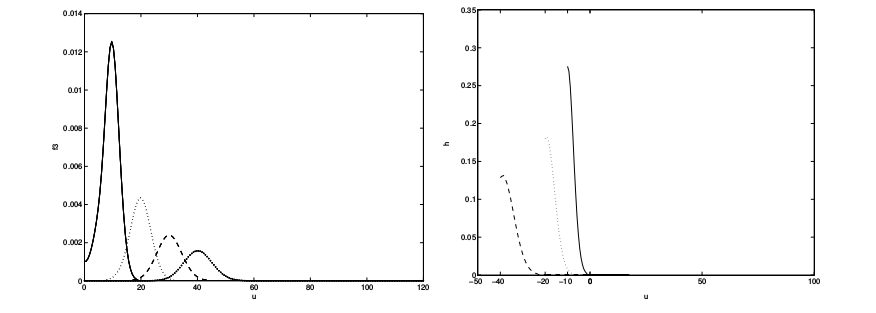
\includegraphics[width=1\textwidth]{test1extension.png}
	\caption{Comportamiento de $f_3$ con $\beta=10$ y condiciones iniciales de caso 1}
	\label{fig:ejemplo5}
\end{figure}
\paragraph{Caso 1:} Consideremos un primer ejemplo de simulaciones numéricas obtenidas con el siguientes conjunto de datos iniciales:
$$A_1 = 0.5, A_2 = 0.2, \beta = 1$$
 Los gráficos de $A_1, A_2 A_3$ (Figura 1-3) muestran cómo se alcanza el comportamiento asintótico descrito en el Teorema (3). El gráfico de $f_3(t, u)$ en el que se representan varios tiempos muestra cómo evolucionan las células tumorales como una especie de ondas viajeras que se mueven desde los valores más bajos de infección tumoral hacia valores más altos. Los gráficos representados a la derecha en la Figura 3 muestran un primer ejemplo de la evolución de la función $h (t, u)$ a medida que aumenta el tiempo, del cual podemos conjetura la forma posible de $L (u)$. También se incluye en la Figura 4,  una representación de como el sistema exhibe un comportamiento similar ante la varianza de $\beta$. Se pueden consultar en \cite{original} otras variaciones de condiciones iniciales que ponen de manifiesto la invarianza del comportamiento cualitativo.
 \paragraph{Caso 2:}
 En este caso elegimos $f_3^0(u)$ como una distribución tipo gaussiana. Como antes escogemos unos parámetros iniciales, que son los mismo que el en caso anterior:
 $$A_1 = 0.5, A_2 = 0.2, \beta = 1$$
 De nuevo el resultado (Figura 5-7) muestra claramente un comportamiento esperado, con las distribuciones tendiendo a resultados concretos y un desarrollo de $f_3$ en ondas que se entiende como incremento de la infección tumoral en tiempo. Además el comportamiento cualitativo también se mantiene bajo variaciones de $\beta$ (Figura 8).
\begin{figure}
	\centering
	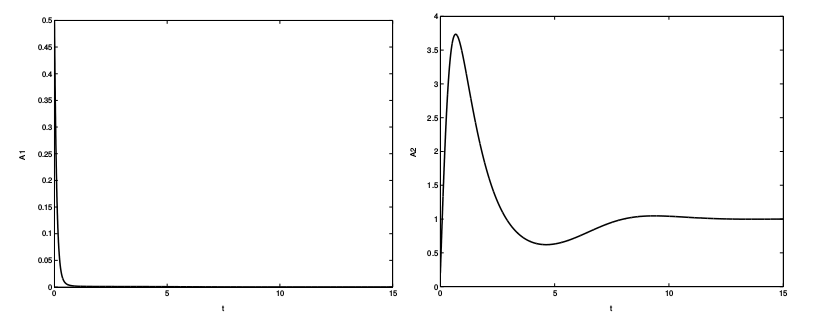
\includegraphics[width=1\textwidth]{test2A1A2.png}
	\caption{Representacion de $A_1$ y $A_2$ en el primer caso}
	\label{fig:ejemplo2}
\end{figure}
\begin{figure}
	\centering
	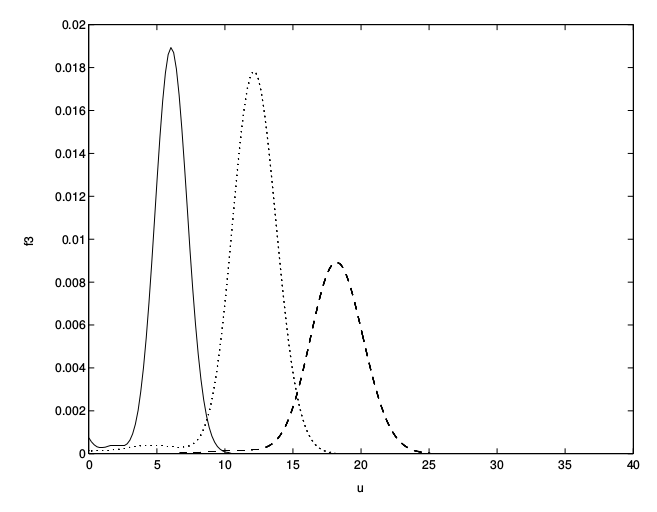
\includegraphics[width=1\textwidth]{test2F3.png}
	\caption{Comportamiento de $f_3$ en el caso 2 las lineas simbolizan la progresión temporal de $t=2$, $t=8$ y $t=14$ }
	\label{fig:ejemplo3}
\end{figure}
\begin{figure}
	\centering
	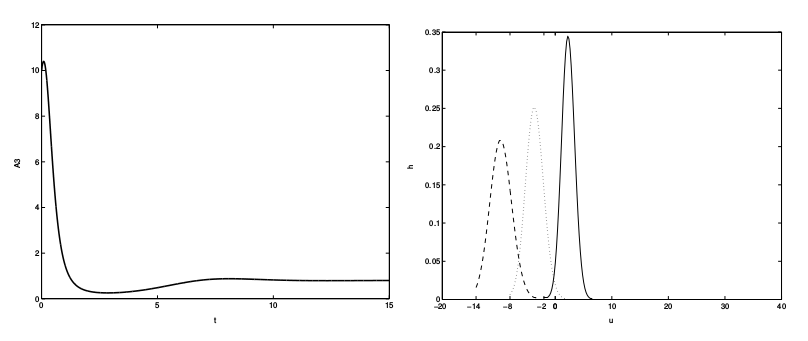
\includegraphics[width=1\textwidth]{test2A3H.png}
	\caption{Comportamiento de $A_3$ y $h$ en el caso 2}
	\label{fig:ejemplo4}
\end{figure}
\begin{figure}
	\centering
	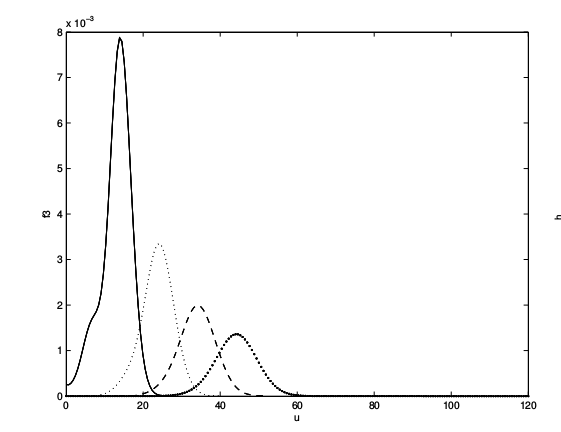
\includegraphics[width=1\textwidth]{test222.png}
	\caption{Comportamiento de $f_3$ con $\beta=10$ y condiciones iniciales de caso 2}
	\label{fig:ejemplo5}
\end{figure}
 
\section{Conclusiones y posibles desarrollos futuros}
Aunque el sistema muestra una desarrollo de $f_3$ en ondas que progresa no en la cantidad, si no en la afección de las células tumorales. Desde un punto de vista biológico, esta situación no puede ser realmente "estable" durante mucho tiempo. Incluso si los períodos de latencia se extienden en cierto punto un sistema real debería evolucionar hacia comportamientos caracterizados, por ejemplo, ya sea por la destrucción total de las células tumorales o por la reactivación del pocas células tumorales con valores de infección muy altos. Tenemos aquí un límite del modelo mismo.

También es destacable la poca reproducibilidad del artículo, sobretodo en cuanto a las simulaciones se refieren.La calidad de los gráficos no es especialmente buena y se podría aportar más información sobre el código para reproducirlo y de ser necesario obtener nuevos gráficos (se han omitido por este motivo los gráficos en 3-D).

Independientemente de esto, me ha parecido muy interesante el enfoque de la teoría cinética de partículas activas a la biología. Para entender correctamente el artículo he tenido que recurrir a otros resultados, no sólo de biología si no de las bases de la teoría cinética de partículas activas en sí misma como \cite{bellomo,libro}. A parte de la visión extensa sobre las posibles aplicaciones de esta teoría, he adquirido conocimiento sobre una gran cantidad de resultados concernientes a la existencia de soluciones y estrategias de modelado que permiten saltar de ámbitos microscópicos a macroscopicos. 

\section*{Referencias}

\bibliography{mybibfile}

\end{document}